\chapter{提案手法}
\thispagestyle{fancy}

\section{使用装置}
\subsection{Kinect for Windows}
Microsoftから販売された,コントローラーを用いずに身体の動き,ジェスチャー,音声などによって
操作を可能にする周辺機器である.

Kinectには,赤外線センサー,8ビット3チャンネル(RGB)の画像データを取得するRGBカメラ,
Kinectからの距離(深度)の画像データを取得する深度画像センサー,音の発生場所を求める
音源位置推定が可能な音声マイクが搭載されている.
また,Kinectの最も特徴的な機能が「姿勢認識技術」である,人間の全身を認識してその動きによる操作をしている.
これにより,深度画像をもとに,人体のパーツがどこにあるのかを推測することができる\cite{kinect}.

本研究では,Kinect for Windows v1を使用した.

\begin{figure}[b]
    \centering
    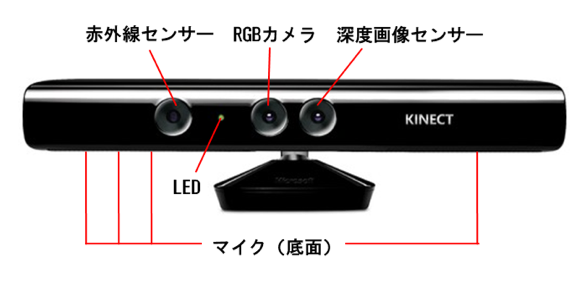
\includegraphics[width=9cm]{image/kinect.png}
    \caption{Kinect for Windows\cite{kinect}}
  \label{kinect}
\end{figure}

\clearpage

\subsection{プロジェクター}
投影を行う際に使用した.


\section{開発環境}

\begin{itemize}
    \item OS: Windows 10
    \item 統合開発環境: Visual Studio 2017
    \item プログラミング言語: C++
    \item ライブラリ: OpenNI2, NiTE2, OpenCV, OpenGL
\end{itemize}

\section{システムの概要}
本研究では,スポーツに焦点を当て野球とサッカーのアクションを行えるプロジェクションマッピングを実装した.


\subsection{骨格座標を用いた手法}
\subsubsection{表示画面}
以下の7つの画面を出力する.

\begin{itemize}
    \item Ball: スポーツで用いるボール
    \item Color: RGBカメラの映像
    \item Depth: 深度カメラの映像
    \item User: 人領域の映像
    \item Combination: 投影用
    \item Combination\_PC: PC用
    \item Skeleton: 人の骨格情報
\end{itemize}

\clearpage

\begin{figure}[p]
    \begin{minipage}{0.5\hsize}
     \begin{center}
      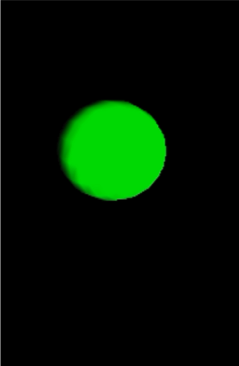
\includegraphics[width=4cm,height=6cm]{image/ball.png}
     \end{center}
     \caption{Ballの画面表示}
     \label{ball}
    \end{minipage}
    \begin{minipage}{0.5\hsize}
     \begin{center}
      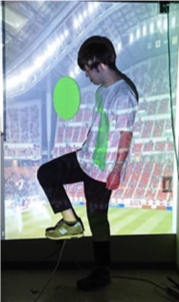
\includegraphics[width=4cm,height=6cm]{image/color.png}
     \end{center}
     \caption{Colorの画面表示}
     \label{color}
    \end{minipage}
\end{figure}

\begin{figure}[p]
    \begin{minipage}{0.5\hsize}
     \begin{center}
      \includegraphics[width=4cm,height=6cm]{image/Depth.png}
     \end{center}
     \caption{Depthの画面表示}
     \label{ball}
    \end{minipage}
    \begin{minipage}{0.5\hsize}
     \begin{center}
      \includegraphics[width=4cm,height=6cm]{image/User.png}
     \end{center}
     \caption{Userの画面表示}
     \label{color}
    \end{minipage}
\end{figure}

\clearpage

\begin{figure}[p]
    \begin{minipage}{0.5\hsize}
     \begin{center}
      \includegraphics[width=4cm,height=6cm]{image/Combination.png}
     \end{center}
     \caption{CombinationとCombination\_PCの画面表示}
     \label{ball}
    \end{minipage}
    \begin{minipage}{0.5\hsize}
     \begin{center}
      \includegraphics[width=4cm,height=6cm]{image/Skeleton.png}
     \end{center}
     \caption{Skeletonの画面表示}
     \label{color}
    \end{minipage}
\end{figure}

\clearpage

\subsubsection{スケルトンナンバーについて}
Kinect v1において,スケルトンは図\ref{num}に示すように番号が割り当てられている.

\begin{figure}[htbp]
    \centering
    \includegraphics[height=7cm]{image/Skeleton_num.png}
    \caption{スケルトンナンバー}
  \label{num}
\end{figure}

\begin{table}[h]
    \centering
    \begin{tabular}{|lc|lc|} \hline
      0 & 頭 & 8 & 胴体 \\ 
      1 & 首 & 9 & 左腰 \\
      2 & 左肩 & 10 & 右腰 \\
      3 & 右肩 & 11 & 左膝 \\
      4 & 左肘 & 12 & 右膝 \\
      5 & 右肘 & 13 & 左足 \\
      6 & 左手 & 14 & 右足 \\
      7 & 右手 &  &  \\ \hline
    \end{tabular}
    \caption{スケルトンナンバーと体の位置関係}
    \label{num}
\end{table}

\clearpage
ほげ

\clearpage
\subsection{物体検出器を用いた手法}